% Created 2024-08-27 Tue 10:14
% Intended LaTeX compiler: pdflatex
\documentclass[11pt]{article}
\usepackage[utf8]{inputenc}
\usepackage[T1]{fontenc}
\usepackage{graphicx}
\usepackage{longtable}
\usepackage{wrapfig}
\usepackage{rotating}
\usepackage[normalem]{ulem}
\usepackage{amsmath}
\usepackage{amssymb}
\usepackage{capt-of}
\usepackage{hyperref}
\setcounter{secnumdepth}{2}
\author{Fabrice Niessen}
\date{\today}
\title{How to effortlessly transform your Org mode files into stunning HTML in just 2 minutes}
\hypersetup{
 pdfauthor={Fabrice Niessen},
 pdftitle={How to effortlessly transform your Org mode files into stunning HTML in just 2 minutes},
 pdfkeywords={org-mode, export, html, theme, style, css, js, bigblow},
 pdfsubject={Org-HTML export made simple.},
 pdfcreator={Emacs 29.4 (Org mode 9.6.28)}, 
 pdflang={English}}
\begin{document}

\maketitle
\tableofcontents


\section{ADVERT: Elevate your Emacs skills in Paris, Rotterdam, Leuven or Valencia!}
\label{sec:org342d1f8}

\textbf{Unlock the power of Emacs in Valencia!  Join my next exclusive "Emacs Boost"
course on April 11th to 12th, 2024!}

\begin{center}
\includegraphics[width=.9\linewidth]{images/Logo-HD-transparent-25pc.png}
\end{center}

Ready to \emph{supercharge your productivity} and become an Emacs ninja?  Look no
further!

\textbf{What you'll learn:}
\begin{itemize}
\item Master Emacs from the basics to advanced tricks.
\item \emph{Boost your editing efficiency} and streamline your workflow.
\item Customize Emacs to fit your unique needs.
\item And much more!
\end{itemize}

\textbf{Upcoming course details:}
\begin{itemize}
\item \textbf{Date:} April 11th to 12th (Thu + Fri)
\item \textbf{Location:} Valencia, Spain
\item \textbf{Audience:} Open to anyone interested in Emacs, from beginners to advanced
users.
\end{itemize}

\textbf{Why choose my course?}
\begin{itemize}
\item Expert instructor with 24 years of Emacs experience.
\item \emph{Hands-on exercises} to reinforce your learning.
\item \emph{Networking opportunities} with like-minded Emacs enthusiasts.
\item Personalized attention.
\end{itemize}

Don't miss this opportunity to take your Emacs skills to the next level! \\[0pt]
Seats are limited, so \emph{reserve yours today}.

Visit \url{https://emacsboost.com/en/} for more information, other dates and other
locations, and to \emph{reserve your seat}.

\emph{See you in Valencia!}  \href{https://emacsboost.com/en/}{\#EmacsBoostValencia}

\section{Overview}
\label{sec:org75a5b9c}

\subsection{Description}
\label{sec:org59eb686}

Though you can easily override CSS stylesheets and add your own HTML themes, we
can say (or write) that Org mode provides a \emph{basic} HTML support.

\textbf{Org-HTML themes} is an open source framework for providing you with a list of
very nice (cross-browser) themes for all your Org documents.  Use them to \textbf{style
your docs}, and your colleagues will come up to tell you that you are a genius!

Share this content by tweeting this page:

Follow \href{https://twitter.com/f\_niessen}{f\textsubscript{niessen}} on Twitter for updates on Org-HTML themes!

\subsection{Requirements}
\label{sec:orgb6b2d60}

Org mode version 8 (or later) is required.

If such a version is not bundled with your Emacs, install one from ELPA.

\section{Gallery}
\label{sec:org5fdcf56}
This is a list of available \textbf{HTML themes for Org mode}, which you can use right
now!

\subsection{Bigblow}
\label{sec:orgd8cf014}

Bigblow is perfect for your work: it is a clean design aimed at optimal \textbf{Org
mode experience in your browser}.  It looks just awesome!

\href{https://www.youtube.com/watch?v=DnSGSiXYuOk}{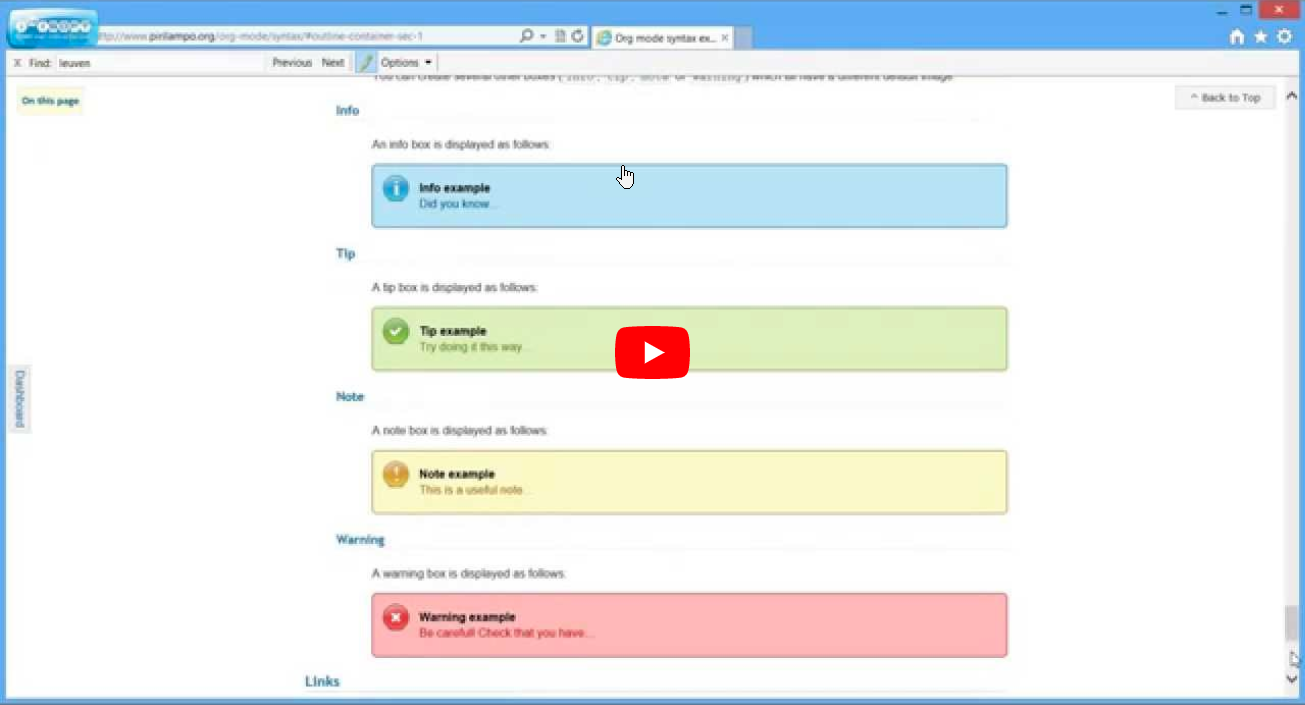
\includegraphics[width=.9\linewidth]{docs/bigblow.png}}

Click on the image for a quick \href{https://www.youtube.com/watch?v=DnSGSiXYuOk}{demo of Bigblow} (2:49 min, no audio).

Keyboard shortcuts to save time and boost your productivity:

\begin{center}
\begin{tabular}{ll}
Shortcut & What it does\\[0pt]
\hline
\texttt{?} or \texttt{h} & Access the \textbf{dashboard}\\[0pt]
\texttt{n} & Move to the \textbf{next} main heading\\[0pt]
\texttt{p} & Move to the \textbf{previous} main heading\\[0pt]
\texttt{b} & Scroll up\\[0pt]
\texttt{<} & Scroll to top\\[0pt]
\texttt{>} & Scroll to bottom\\[0pt]
\texttt{-} & Collapse all\\[0pt]
\texttt{+} & Expand all\\[0pt]
\texttt{r} & Go to next task in list\\[0pt]
\texttt{R} & Go to previous task in list\\[0pt]
\texttt{q} & Stop reviewing the list of tasks\\[0pt]
\texttt{g} & Reload the page\\[0pt]
\end{tabular}
\end{center}

\subsubsection*{Quotations about Bigblow}
\label{sec:org1a76c89}

"Very very nice, I enjoy it a lot." \\[0pt]
-- \emph{Ista Zahn}

"This is awesome.  I love it!" \\[0pt]
-- \emph{Rainer M Krug}

"This is awesome!!" \\[0pt]
-- \emph{Mehul Sanghvi}

"This very nice html theme. [\ldots{}]  I cannot use another emacs-theme than your
\href{https://github.com/fniessen/emacs-leuven-theme}{emacs-leuven-theme}, and it is going to be probably the same with your html
theme!" \\[0pt]
-- \emph{Joseph Vidal-Rosset}

"Thanks a lot for sharing [\ldots{}] the wonderful Bigblow theme.  I create lot of
specification for other team members to use.  It has always been a trouble to
share and maintain such spec.  Now, I can create a much neater spec which is
available for the team's reference as a webpage." \\[0pt]
-- \emph{Shankar R.}

"I like Bigblow the best.  I've exported most of my Org files using this theme
and published them within my company's intranet.  Thanks for sharing this
wonderful package!" \\[0pt]
-- \emph{Richard K.}

\subsection{ReadTheOrg}
\label{sec:org8e6932a}

ReadTheOrg is a clone of the official -- and great! -- \href{https://github.com/snide/sphinx\_rtd\_theme}{Sphinx theme} used in the
\href{http://docs.readthedocs.org/en/latest/}{Read The Docs} site.  It gives a beautiful and professional style to all your Org
docs.

\textbf{Thanks to its creator(s)!}

\begin{center}
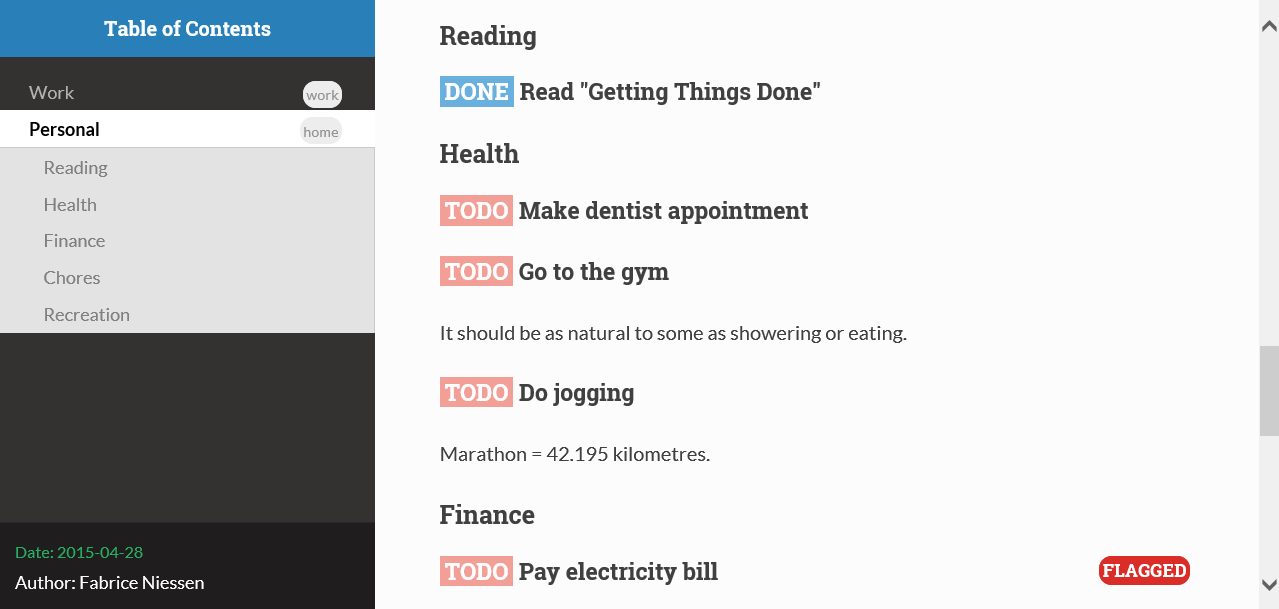
\includegraphics[width=.9\linewidth]{docs/readtheorg.png}
\end{center}

\begin{note}
While the original theme shines on mobile devices as well, ReadTheOrg does not
stay completely functional.

I don't have a lot of time to maintain this project due to other
responsibilities.  Help is welcome to work on that (and eventually improve the
default structure of the HTML export)!
\end{note}

\subsubsection*{Quotations about ReadTheOrg}
\label{sec:org1b4c328}

"OMG.  The ReadTheOrg theme for exported HTML from org mode files is eye
wateringly beautiful.  Thank you!" \\[0pt]
-- \emph{Rob Stewart}

"It is fantastic, so beautiful.  I will switch several of my pages over to
this theme." \\[0pt]
-- \emph{Carsten D.}

"That is incredibly impressive.  Thanks for this." \\[0pt]
-- \emph{Noah R.}

"Thank you!  I enjoy your themes.  The best ones I've ever found." \\[0pt]
-- \emph{Kang T.}

"Awesome theme.  Wonderful job.  You're doing a wonderful thing --- it will
enable people (at least those who use Emacs and Org mode) to put together
on-line reference works in a much-more usable fashion than is currently
available." \\[0pt]
-- \emph{D. C. Toedt}

"Extremely useful." \\[0pt]
-- \emph{Thomas S. Dye}

"This is amazing, I've been looking for something like this for a LONG time!
I will share." \\[0pt]
-- \emph{Edward H.}

\section{Demo}
\label{sec:org492cf41}

I've written a \href{tests/org-mode-syntax-example.org}{demo page} for the themes that provides a maximal working support
of Org mode syntax.

Please see the \href{https://github.com/fniessen/refcard-org-mode}{Org mode refcard} page for full examples of headings, code,
admonitions, footnotes, tables and other details.

\section{Using a theme}
\label{sec:org6638272}

Using a theme from the \hyperref[sec:org5fdcf56]{theme gallery} for your own Org documents is very easy:

\begin{enumerate}
\item You \textbf{add a} \texttt{\#+SETUPFILE:} \textbf{directive} in the preamble of your document (to include
the necessary CSS and JavaScript files).

You can either use an URL of the following type for the "setup file" of your
chosen theme:

\begin{verbatim}
#+SETUPFILE: https://fniessen.github.io/org-html-themes/org/theme-NAME.setup
\end{verbatim}

(where \texttt{NAME} is either \texttt{bigblow} or \texttt{readtheorg})

or, if you \textbf{cloned or downloaded} the Org-HTML themes project -- to get no
dependency on an Internet connection --, use a (relative or absolute) path to
the \emph{local} "setup file" and copy the \texttt{src} folder from the cloned folder
into the same folder as the file you want to export:

\begin{verbatim}
#+SETUPFILE: PATH/TO/GIT/REPO/org/theme-NAME-local.setup
\end{verbatim}

\item Then, you \textbf{export} your Org mode file \textbf{to HTML} with \texttt{org-html-export-to-html} or
with \texttt{C-c C-e h h}.
\end{enumerate}

\section{Customizing a theme}
\label{sec:org080523d}

You love those themes, but you still would like to override particular HTML
tags?  Some examples do follow\ldots{}

Before doing that, though, if you think it really is an improvement that could
serve other persons as well, including me, you're invited to submit your
change\ldots{}

\subsection{Change the background code blocks}
\label{sec:orge9f859e}

Here's an example to insert into your Org documents:

\begin{verbatim}
# Change the background of source block.
#+HTML_HEAD: <style>pre.src{background:#343131;color:white;} </style>
\end{verbatim}

\subsection{Unset body width limit of ReadTheOrg}
\label{sec:org7404cf5}

Solution provided by Malcolm Cook:

\begin{verbatim}
#+HTML_HEAD: <style> #content{max-width:1800px;}</style>
#+HTML_HEAD: <style> p{max-width:800px;}</style>
#+HTML_HEAD: <style> li{max-width:800px;}</style
\end{verbatim}

\section{Contribute to the project!}
\label{sec:orgddfd2f3}

\subsection{Report issues and enhancements}
\label{sec:org0eb6a6c}

Found a bug or have an idea for a new feature?  Share your thoughts on the
\href{https://github.com/fniessen/org-html-themes/issues/new}{GitHub issue tracker}.

\subsection{Submit patches}
\label{sec:orge8223db}

I welcome contributions in any form!  Feel free to submit patches to enhance the
project.

\subsection{Support development with a donation!}
\label{sec:orgff81331}

If you find the "org-html-themes" project (or any of \href{https://github.com/fniessen/}{my other projects})
enhancing your Emacs experience and simplifying your workflow, seize the
opportunity to express your appreciation!  Help fuel future development by
making a \href{https://www.paypal.com/cgi-bin/webscr?cmd=\_donations\&business=VCVAS6KPDQ4JC\&lc=BE\&item\_number=org\%2dhtml\%2dthemes\&currency\_code=EUR\&bn=PP\%2dDonationsBF\%3abtn\_donate\_LG\%2egif\%3aNonHosted}{donation} through PayPal. Your support is invaluable -- thank you!

Remember, regardless of donations, "org-html-themes" will always remain freely
accessible, both as in Belgian beer and as in speech.

\section{License}
\label{sec:org1d0a147}

Copyright (C) 2011-2024 Fabrice Niessen

Author: Fabrice Niessen \\[0pt]
Keywords: org-mode html themes

This program is free software; you can redistribute it and/or modify it under
the terms of the GNU General Public License as published by the Free Software
Foundation, either version 3 of the License, or (at your option) any later
version.

This program is distributed in the hope that it will be useful, but WITHOUT ANY
WARRANTY; without even the implied warranty of MERCHANTABILITY or FITNESS FOR
A PARTICULAR PURPOSE.  See the GNU General Public License for more details.

You should have received a copy of the GNU General Public License along with
this program.  If not, see \url{http://www.gnu.org/licenses/}.
\end{document}
